\documentclass{standalone}
\usepackage{tikz}
\usetikzlibrary{patterns, positioning}
\usepackage[sfdefault]{ClearSans} %% option 'sfdefault' activates Clear Sans as the default text font
\usepackage[T1]{fontenc}

\begin{document}
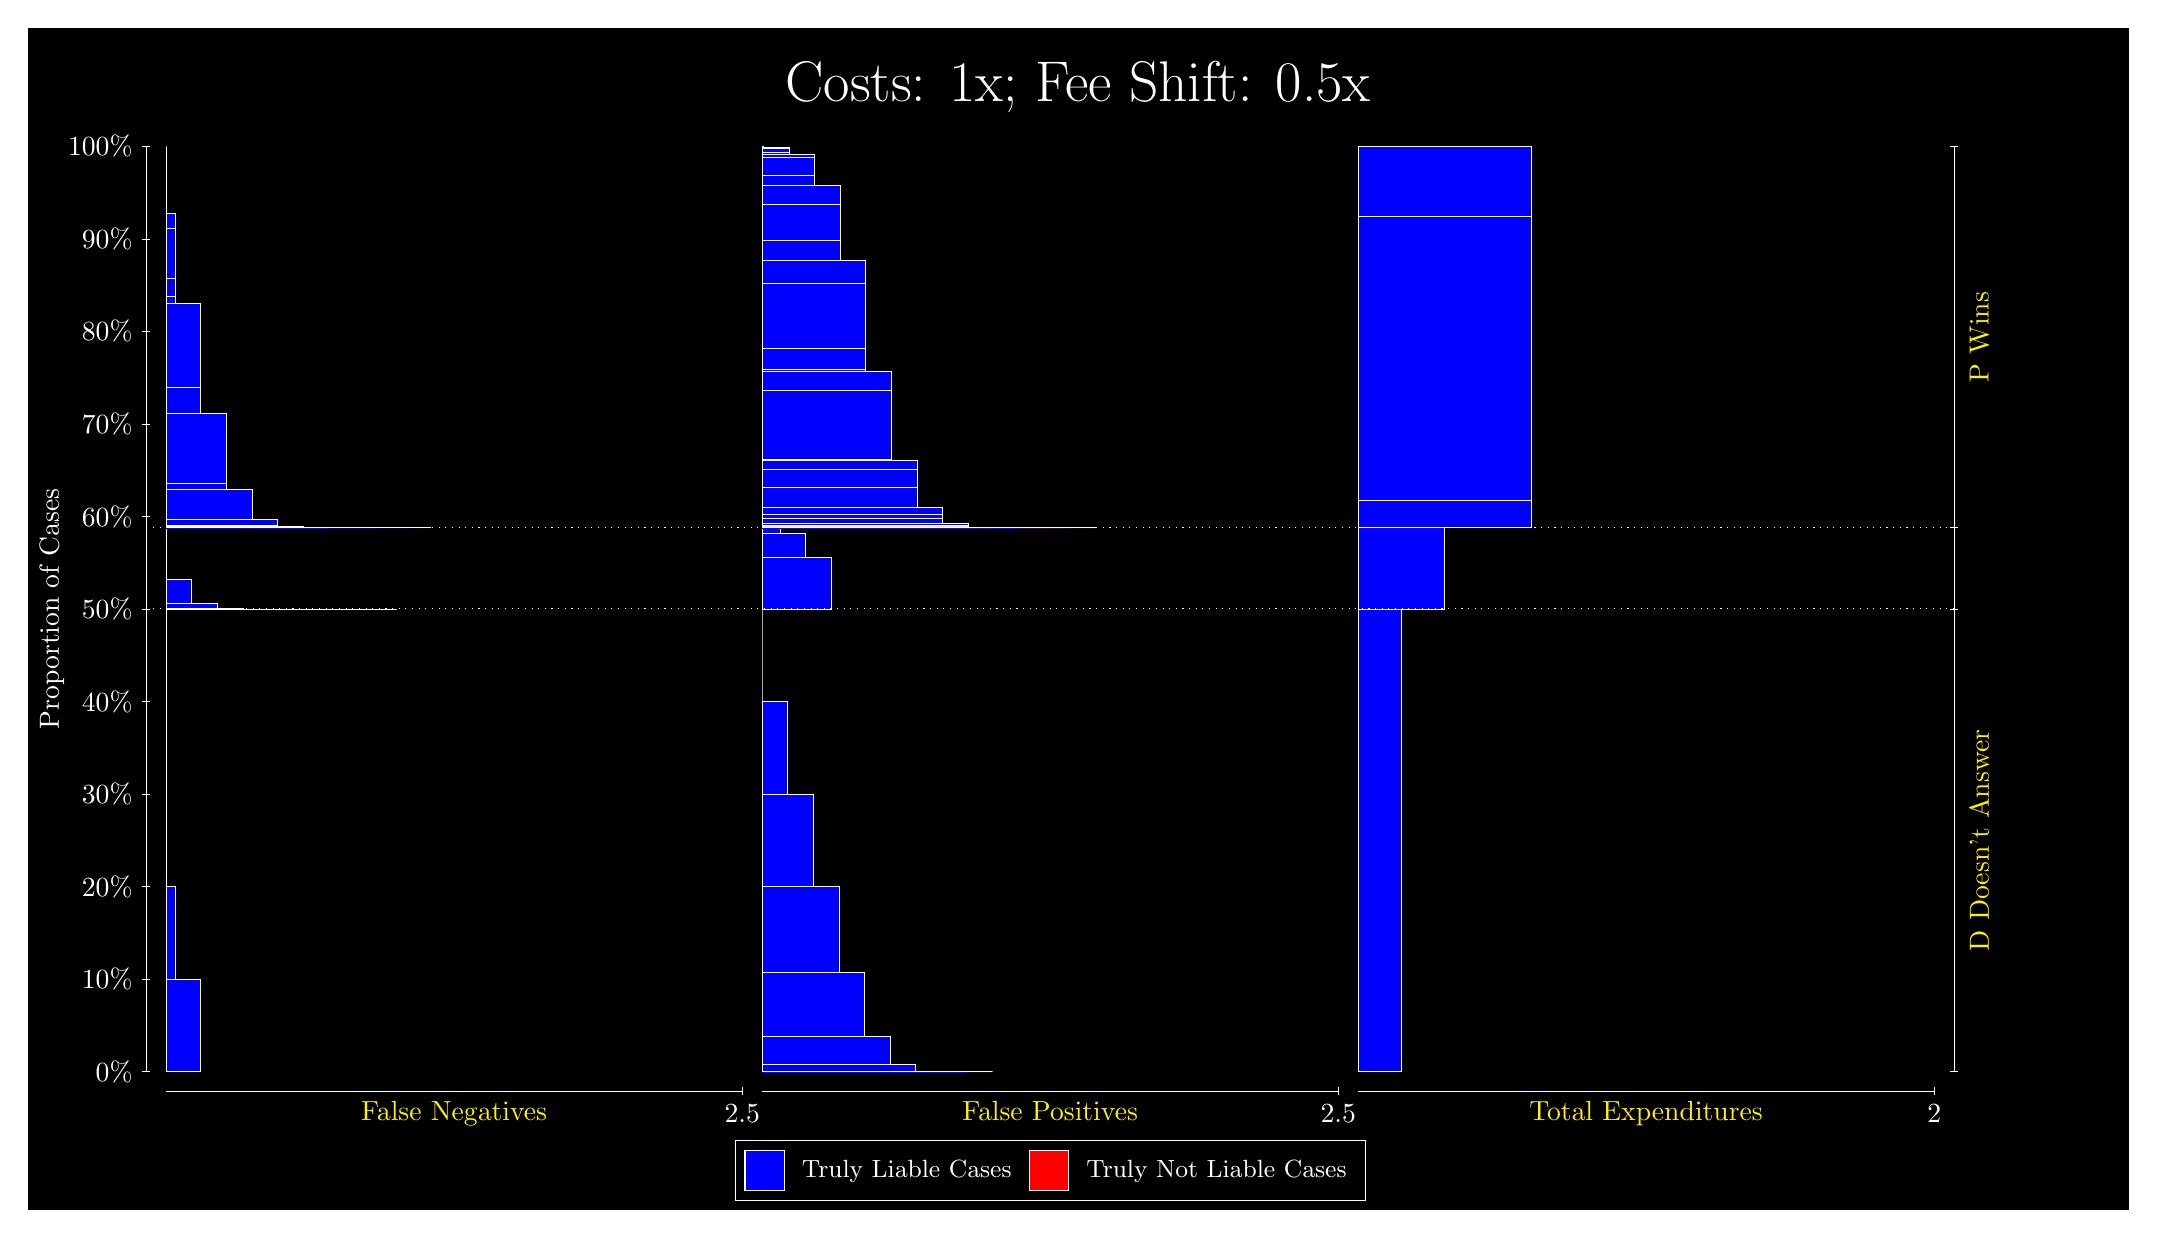
\begin{tikzpicture}
\draw[fill=black] (0,0) rectangle (26.667,15);
\draw[text=white] (0,13.5) rectangle (26.667,15) node[midway] {\huge Costs: 1x; Fee Shift: 0.5x};
\draw[white, very thin] (1.5,1.75) -- (1.5,13.5);
\node[rotate=90, text=white, anchor=center] at (0.3, 7.625) {Proportion of Cases};
\draw[white, very thin] (1.45,1.75) -- (1.55,1.75);
\node[text=white, anchor=east] at (1.45, 1.75) {0\%};
\draw[white, very thin] (1.45,2.925) -- (1.55,2.925);
\node[text=white, anchor=east] at (1.45, 2.925) {10\%};
\draw[white, very thin] (1.45,4.1) -- (1.55,4.1);
\node[text=white, anchor=east] at (1.45, 4.1) {20\%};
\draw[white, very thin] (1.45,5.275) -- (1.55,5.275);
\node[text=white, anchor=east] at (1.45, 5.275) {30\%};
\draw[white, very thin] (1.45,6.45) -- (1.55,6.45);
\node[text=white, anchor=east] at (1.45, 6.45) {40\%};
\draw[white, very thin] (1.45,7.625) -- (1.55,7.625);
\node[text=white, anchor=east] at (1.45, 7.625) {50\%};
\draw[white, very thin] (1.45,8.8) -- (1.55,8.8);
\node[text=white, anchor=east] at (1.45, 8.8) {60\%};
\draw[white, very thin] (1.45,9.975) -- (1.55,9.975);
\node[text=white, anchor=east] at (1.45, 9.975) {70\%};
\draw[white, very thin] (1.45,11.15) -- (1.55,11.15);
\node[text=white, anchor=east] at (1.45, 11.15) {80\%};
\draw[white, very thin] (1.45,12.325) -- (1.55,12.325);
\node[text=white, anchor=east] at (1.45, 12.325) {90\%};
\draw[white, very thin] (1.45,13.5) -- (1.55,13.5);
\node[text=white, anchor=east] at (1.45, 13.5) {100\%};

\draw[white, very thin] (24.457,1.75) -- (24.457,13.5);
\draw[white, very thin] (24.407,1.75) -- (24.507,1.75);
\node[anchor=west] at (24.407, 1.75) {};
\draw[white, very thin] (24.407,7.625) -- (24.507,7.625);
\node[anchor=west] at (24.407, 7.625) {};
\draw[white, very thin] (24.407,8.6579) -- (24.507,8.6579);
\node[anchor=west] at (24.407, 8.6579) {};
\draw[white, very thin] (24.407,13.5) -- (24.507,13.5);
\node[anchor=west] at (24.407, 13.5) {};

\draw[white, very thin, fill=blue] (1.75,1.75) rectangle (2.1891,2.925);
\draw[white, very thin, fill=blue] (1.75,2.925) rectangle (1.8638,4.0997);
\draw[white, very thin, fill=red] (1.75,4.0997) rectangle (1.75,4.0997);
\draw[white, very thin, fill=blue] (1.75,4.0997) rectangle (1.75,7.625);
\draw[white, very thin, fill=blue] (1.75,7.625) rectangle (4.6775,7.625);
\draw[white, very thin, fill=blue] (1.75,7.625) rectangle (4.3523,7.625);
\draw[white, very thin, fill=blue] (1.75,7.625) rectangle (4.027,7.625);
\draw[white, very thin, fill=blue] (1.75,7.625) rectangle (3.7017,7.625);
\draw[white, very thin, fill=blue] (1.75,7.625) rectangle (3.3764,7.625);
\draw[white, very thin, fill=blue] (1.75,7.625) rectangle (3.0511,7.6252);
\draw[white, very thin, fill=blue] (1.75,7.6252) rectangle (2.7258,7.6318);
\draw[white, very thin, fill=blue] (1.75,7.6318) rectangle (2.4006,7.703);
\draw[white, very thin, fill=blue] (1.75,7.703) rectangle (2.0753,8.0073);
\draw[white, very thin, fill=red] (1.75,8.0073) rectangle (1.75,8.0073);
\draw[white, very thin, fill=blue] (1.75,8.0073) rectangle (1.75,8.6579);
\draw[white, very thin, fill=blue] (1.75,8.6579) rectangle (5.1167,8.6579);
\draw[white, very thin, fill=blue] (1.75,8.6579) rectangle (4.7914,8.6579);
\draw[white, very thin, fill=blue] (1.75,8.6579) rectangle (4.7914,8.6579);
\draw[white, very thin, fill=blue] (1.75,8.6579) rectangle (4.4661,8.6579);
\draw[white, very thin, fill=blue] (1.75,8.6579) rectangle (4.4661,8.6579);
\draw[white, very thin, fill=blue] (1.75,8.6579) rectangle (4.1408,8.658);
\draw[white, very thin, fill=blue] (1.75,8.658) rectangle (3.8155,8.6584);
\draw[white, very thin, fill=blue] (1.75,8.6584) rectangle (3.8155,8.6585);
\draw[white, very thin, fill=blue] (1.75,8.6585) rectangle (3.4903,8.6692);
\draw[white, very thin, fill=blue] (1.75,8.6692) rectangle (3.165,8.6833);
\draw[white, very thin, fill=blue] (1.75,8.6833) rectangle (3.165,8.759);
\draw[white, very thin, fill=blue] (1.75,8.759) rectangle (2.8397,9.1488);
\draw[white, very thin, fill=blue] (1.75,9.1488) rectangle (2.5144,9.227);
\draw[white, very thin, fill=blue] (1.75,9.227) rectangle (2.5144,10.108);
\draw[white, very thin, fill=blue] (1.75,10.108) rectangle (2.1891,10.438);
\draw[white, very thin, fill=blue] (1.75,10.438) rectangle (2.1891,11.513);
\draw[white, very thin, fill=blue] (1.75,11.513) rectangle (1.8638,11.592);
\draw[white, very thin, fill=blue] (1.75,11.592) rectangle (1.8638,11.824);
\draw[white, very thin, fill=blue] (1.75,11.824) rectangle (1.8638,12.46);
\draw[white, very thin, fill=blue] (1.75,12.46) rectangle (1.8638,12.648);
\draw[white, very thin, fill=red] (1.75,12.648) rectangle (1.75,12.648);
\draw[white, very thin, fill=blue] (1.75,12.648) rectangle (1.75,13.5);
\draw[white, very thin, fill=red] (9.3189,1.75) rectangle (12.246,1.75);
\draw[white, very thin, fill=blue] (9.3189,1.75) rectangle (12.246,1.75);
\draw[white, very thin, fill=blue] (9.3189,1.75) rectangle (11.921,1.7503);
\draw[white, very thin, fill=blue] (9.3189,1.7503) rectangle (11.596,1.7576);
\draw[white, very thin, fill=blue] (9.3189,1.7576) rectangle (11.271,1.8362);
\draw[white, very thin, fill=blue] (9.3189,1.8362) rectangle (10.945,2.1987);
\draw[white, very thin, fill=blue] (9.3189,2.1987) rectangle (10.62,3.0112);
\draw[white, very thin, fill=blue] (9.3189,3.0112) rectangle (10.295,4.1076);
\draw[white, very thin, fill=blue] (9.3189,4.1076) rectangle (9.9694,5.2753);
\draw[white, very thin, fill=blue] (9.3189,5.2753) rectangle (9.6442,6.45);
\draw[white, very thin, fill=blue] (9.3189,6.45) rectangle (9.3189,7.625);
\draw[white, very thin, fill=red] (9.3189,7.625) rectangle (10.197,7.625);
\draw[white, very thin, fill=blue] (9.3189,7.625) rectangle (10.197,8.2757);
\draw[white, very thin, fill=blue] (9.3189,8.2757) rectangle (9.8718,8.58);
\draw[white, very thin, fill=blue] (9.3189,8.58) rectangle (9.5466,8.6512);
\draw[white, very thin, fill=blue] (9.3189,8.6512) rectangle (9.3189,8.6579);
\draw[white, very thin, fill=red] (9.3189,8.6579) rectangle (13.564,8.6579);
\draw[white, very thin, fill=blue] (9.3189,8.6579) rectangle (13.564,8.6579);
\draw[white, very thin, fill=red] (9.3189,8.6579) rectangle (13.239,8.6579);
\draw[white, very thin, fill=blue] (9.3189,8.6579) rectangle (13.239,8.658);
\draw[white, very thin, fill=red] (9.3189,8.658) rectangle (12.913,8.658);
\draw[white, very thin, fill=blue] (9.3189,8.658) rectangle (12.913,8.658);
\draw[white, very thin, fill=blue] (9.3189,8.658) rectangle (12.913,8.658);
\draw[white, very thin, fill=red] (9.3189,8.658) rectangle (12.588,8.658);
\draw[white, very thin, fill=blue] (9.3189,8.658) rectangle (12.588,8.6584);
\draw[white, very thin, fill=red] (9.3189,8.6584) rectangle (12.263,8.6584);
\draw[white, very thin, fill=blue] (9.3189,8.6584) rectangle (12.263,8.6645);
\draw[white, very thin, fill=blue] (9.3189,8.6645) rectangle (11.937,8.6738);
\draw[white, very thin, fill=blue] (9.3189,8.6738) rectangle (11.937,8.6836);
\draw[white, very thin, fill=red] (9.3189,8.6836) rectangle (11.937,8.6836);
\draw[white, very thin, fill=blue] (9.3189,8.6836) rectangle (11.937,8.7093);
\draw[white, very thin, fill=blue] (9.3189,8.7093) rectangle (11.612,8.782);
\draw[white, very thin, fill=blue] (9.3189,8.782) rectangle (11.612,8.8288);
\draw[white, very thin, fill=red] (9.3189,8.8288) rectangle (11.612,8.8288);
\draw[white, very thin, fill=blue] (9.3189,8.8288) rectangle (11.612,8.9134);
\draw[white, very thin, fill=blue] (9.3189,8.9134) rectangle (11.287,9.1659);
\draw[white, very thin, fill=red] (9.3189,9.1659) rectangle (11.287,9.1659);
\draw[white, very thin, fill=blue] (9.3189,9.1659) rectangle (11.287,9.3954);
\draw[white, very thin, fill=blue] (9.3189,9.3954) rectangle (11.287,9.5101);
\draw[white, very thin, fill=blue] (9.3189,9.5101) rectangle (10.962,9.5268);
\draw[white, very thin, fill=red] (9.3189,9.5268) rectangle (10.962,9.5268);
\draw[white, very thin, fill=blue] (9.3189,9.5268) rectangle (10.962,10.4);
\draw[white, very thin, fill=blue] (9.3189,10.4) rectangle (10.962,10.645);
\draw[white, very thin, fill=blue] (9.3189,10.645) rectangle (10.636,10.667);
\draw[white, very thin, fill=blue] (9.3189,10.667) rectangle (10.636,10.937);
\draw[white, very thin, fill=red] (9.3189,10.937) rectangle (10.636,10.937);
\draw[white, very thin, fill=blue] (9.3189,10.937) rectangle (10.636,11.762);
\draw[white, very thin, fill=blue] (9.3189,11.762) rectangle (10.636,12.05);
\draw[white, very thin, fill=blue] (9.3189,12.05) rectangle (10.311,12.05);
\draw[white, very thin, fill=blue] (9.3189,12.05) rectangle (10.311,12.311);
\draw[white, very thin, fill=blue] (9.3189,12.311) rectangle (10.311,12.761);
\draw[white, very thin, fill=blue] (9.3189,12.761) rectangle (10.311,13.009);
\draw[white, very thin, fill=blue] (9.3189,13.009) rectangle (9.9857,13.009);
\draw[white, very thin, fill=blue] (9.3189,13.009) rectangle (9.9857,13.131);
\draw[white, very thin, fill=blue] (9.3189,13.131) rectangle (9.9857,13.359);
\draw[white, very thin, fill=blue] (9.3189,13.359) rectangle (9.9857,13.399);
\draw[white, very thin, fill=blue] (9.3189,13.399) rectangle (9.6604,13.43);
\draw[white, very thin, fill=blue] (9.3189,13.43) rectangle (9.6604,13.472);
\draw[white, very thin, fill=blue] (9.3189,13.472) rectangle (9.6604,13.489);
\draw[white, very thin, fill=blue] (9.3189,13.489) rectangle (9.3351,13.499);
\draw[white, very thin, fill=blue] (9.3189,13.499) rectangle (9.3351,13.499);
\draw[white, very thin, fill=blue] (9.3189,13.499) rectangle (9.3189,13.5);
\draw[white, very thin, fill=red] (16.888,1.75) rectangle (17.437,1.75);
\draw[white, very thin, fill=blue] (16.888,1.75) rectangle (17.437,7.625);
\draw[white, very thin, fill=red] (16.888,7.625) rectangle (17.986,7.625);
\draw[white, very thin, fill=blue] (16.888,7.625) rectangle (17.986,8.6579);
\draw[white, very thin, fill=red] (16.888,8.6579) rectangle (19.083,8.6579);
\draw[white, very thin, fill=blue] (16.888,8.6579) rectangle (19.083,9.0007);
\draw[white, very thin, fill=red] (16.888,9.0007) rectangle (19.083,9.0007);
\draw[white, very thin, fill=blue] (16.888,9.0007) rectangle (19.083,12.609);
\draw[white, very thin, fill=red] (16.888,12.609) rectangle (19.083,12.609);
\draw[white, very thin, fill=blue] (16.888,12.609) rectangle (19.083,13.5);
\draw[white, dotted] (1.5,7.625) -- (24.457,7.625);
\draw[white, dotted] (1.5,8.6579) -- (24.457,8.6579);
\draw[white, very thin] (1.75,1.5) -- (9.0689,1.5);
\node[text=yellow, anchor=north] at (5.4094, 1.5) {False Negatives};
\draw[white, very thin] (9.0689,1.45) -- (9.0689,1.55);
\node[text=white, anchor=north] at (9.0689, 1.45) {2.5};

\draw[white, very thin] (9.3189,1.5) -- (16.638,1.5);
\node[text=yellow, anchor=north] at (12.978, 1.5) {False Positives};
\draw[white, very thin] (16.638,1.45) -- (16.638,1.55);
\node[text=white, anchor=north] at (16.638, 1.45) {2.5};

\draw[white, very thin] (16.888,1.5) -- (24.207,1.5);
\node[text=yellow, anchor=north] at (20.547, 1.5) {Total Expenditures};
\draw[white, very thin] (24.207,1.45) -- (24.207,1.55);
\node[text=white, anchor=north] at (24.207, 1.45) {2};

\node[text=yellow, centered, rotate=90] at (24.777, 4.6875) {D Doesn't Answer};

\node[text=yellow, centered, rotate=90] at (24.777, 11.079) {P Wins};

\draw (12.978300999999998,1.5) node[draw=none] (baseCoordinate) {};
\begin{scope}[align=center]
        \matrix[scale=0.5, draw=white, below=0.5cm of baseCoordinate, nodes={draw}, column sep=0.1cm]{
            \node[rectangle, draw, minimum width=0.5cm, minimum height=0.5cm, fill=blue] {}; &
            \node[draw=none, font=\small, text=white] (B) {Truly Liable Cases}; &
            \node[rectangle, draw, minimum width=0.5cm, minimum height=0.5cm, fill=red] {}; &
            \node[draw=none, font=\small, text=white] (B) {Truly Not Liable Cases}; \\
            };
\end{scope}

\end{tikzpicture}
\end{document}